\documentclass[
	a4paper,
	parskip
]{scrartcl}

\usepackage[english]{babel}
\usepackage{authblk}
\usepackage{amsthm}
\usepackage{amsmath}
\usepackage{amssymb}
\usepackage{booktabs}
\usepackage{float}
\usepackage{multirow}
\usepackage{physics}
\usepackage{siunitx}
\usepackage{hyperref}
\usepackage{cleveref}
\usepackage{subcaption}
\usepackage[
  backend=biber,
  sorting=none
]{biblatex}
\usepackage[american]{circuitikz}
\usepackage{glossaries}

\addbibresource{literature.bib}

\makeglossaries
\newglossaryentry{s5990}{name=S5990, description={Hamamatsu two-dimensional PSD}}
\newacronym{psd}{PSD}{position-sensitive detector}

\title{Position-sensitive device}
\author{Bodo Kaiser}
\affil{Ludwig-Maximilians-Universität München}
\affil{\textit{bodo.kaiser@physik.uni-muenchen.de}}

\begin{document}

\maketitle
\tableofcontents

\section{Introduction}

We define a position-sensitive device as a device that outputs voltages proportional to the center of mass coordinates of a light beam incident on a sensitive area.

The present document summarizes the insights acquired on the journey of building such a device.

\subsection{Motivation}

Position-sensitive devices are used in a wide range of industrial and commercial applications, including displacement sensing and beam alignment, see Ref.~\cite[p.~22]{Maekynen00}.

We are interested in using a position-sensitive device for beam pointing alignment in our quantum optics laboratory.

The beam pointing refers to a laser beam's spatial focus and can change through thermal and mechanical effects.
Uncompensated changes in beam alignment can quickly degrade the overall performance of an optical system.
Therefore, it is crucial to align the beam pointing to ensure the optical system's proper operation at hand.

\subsection{Overview}

This document is organized as follows.

The first two sections introduce the theory of the (position-sensitive) photodiode and the operational amplifier.
These sections are rather elaborate and should be skipped by the pragmatic scientist.

The third section describes the (electrical) schematics of the detector.
If you want to adjust parameters, e.g., gain or bandwidth, you should read these sections.

The fourth section is the only significant section if you want to build a \gls{psd}.
If you also want an example of using the \gls{psd} in an optical setup to determine the spatial resolution, you should also read the fifth section.
Finally, the appendix gives some guidance on troubleshooting.

\subsection{Requirements}

The requirements are specified rather loose. The only hard requirement concerns the connectors and voltages of the power supply. The power connector should be a LEMO4 whose pin configuration is compatible with the \SI{\pm15}{\volt} dual-voltage power supplies used in the labs. Features that would be nice to have are:
\begin{enumerate}
	\item The device should be sensible with optical powers that are safe to operate, i.e., $P<\SI{1}{\micro\watt}$. There is no preferred wavelength.
	\item For easy integration into existing optical setups, the device should be as compact as possible. Additional space, if needed, should be occupied by elonging the height. The sensitive area of the detector should be on the bottom. The connectors should be on the top to avoid cables blocking the beam path.
	\item It should be possible to mount different detector sizes on the device.
\end{enumerate}
The range of the output voltages of the device can be chosen for the optimal signal-to-noise ratio.

\subsection{Specification}

\begin{figure}[H]
	\centering
	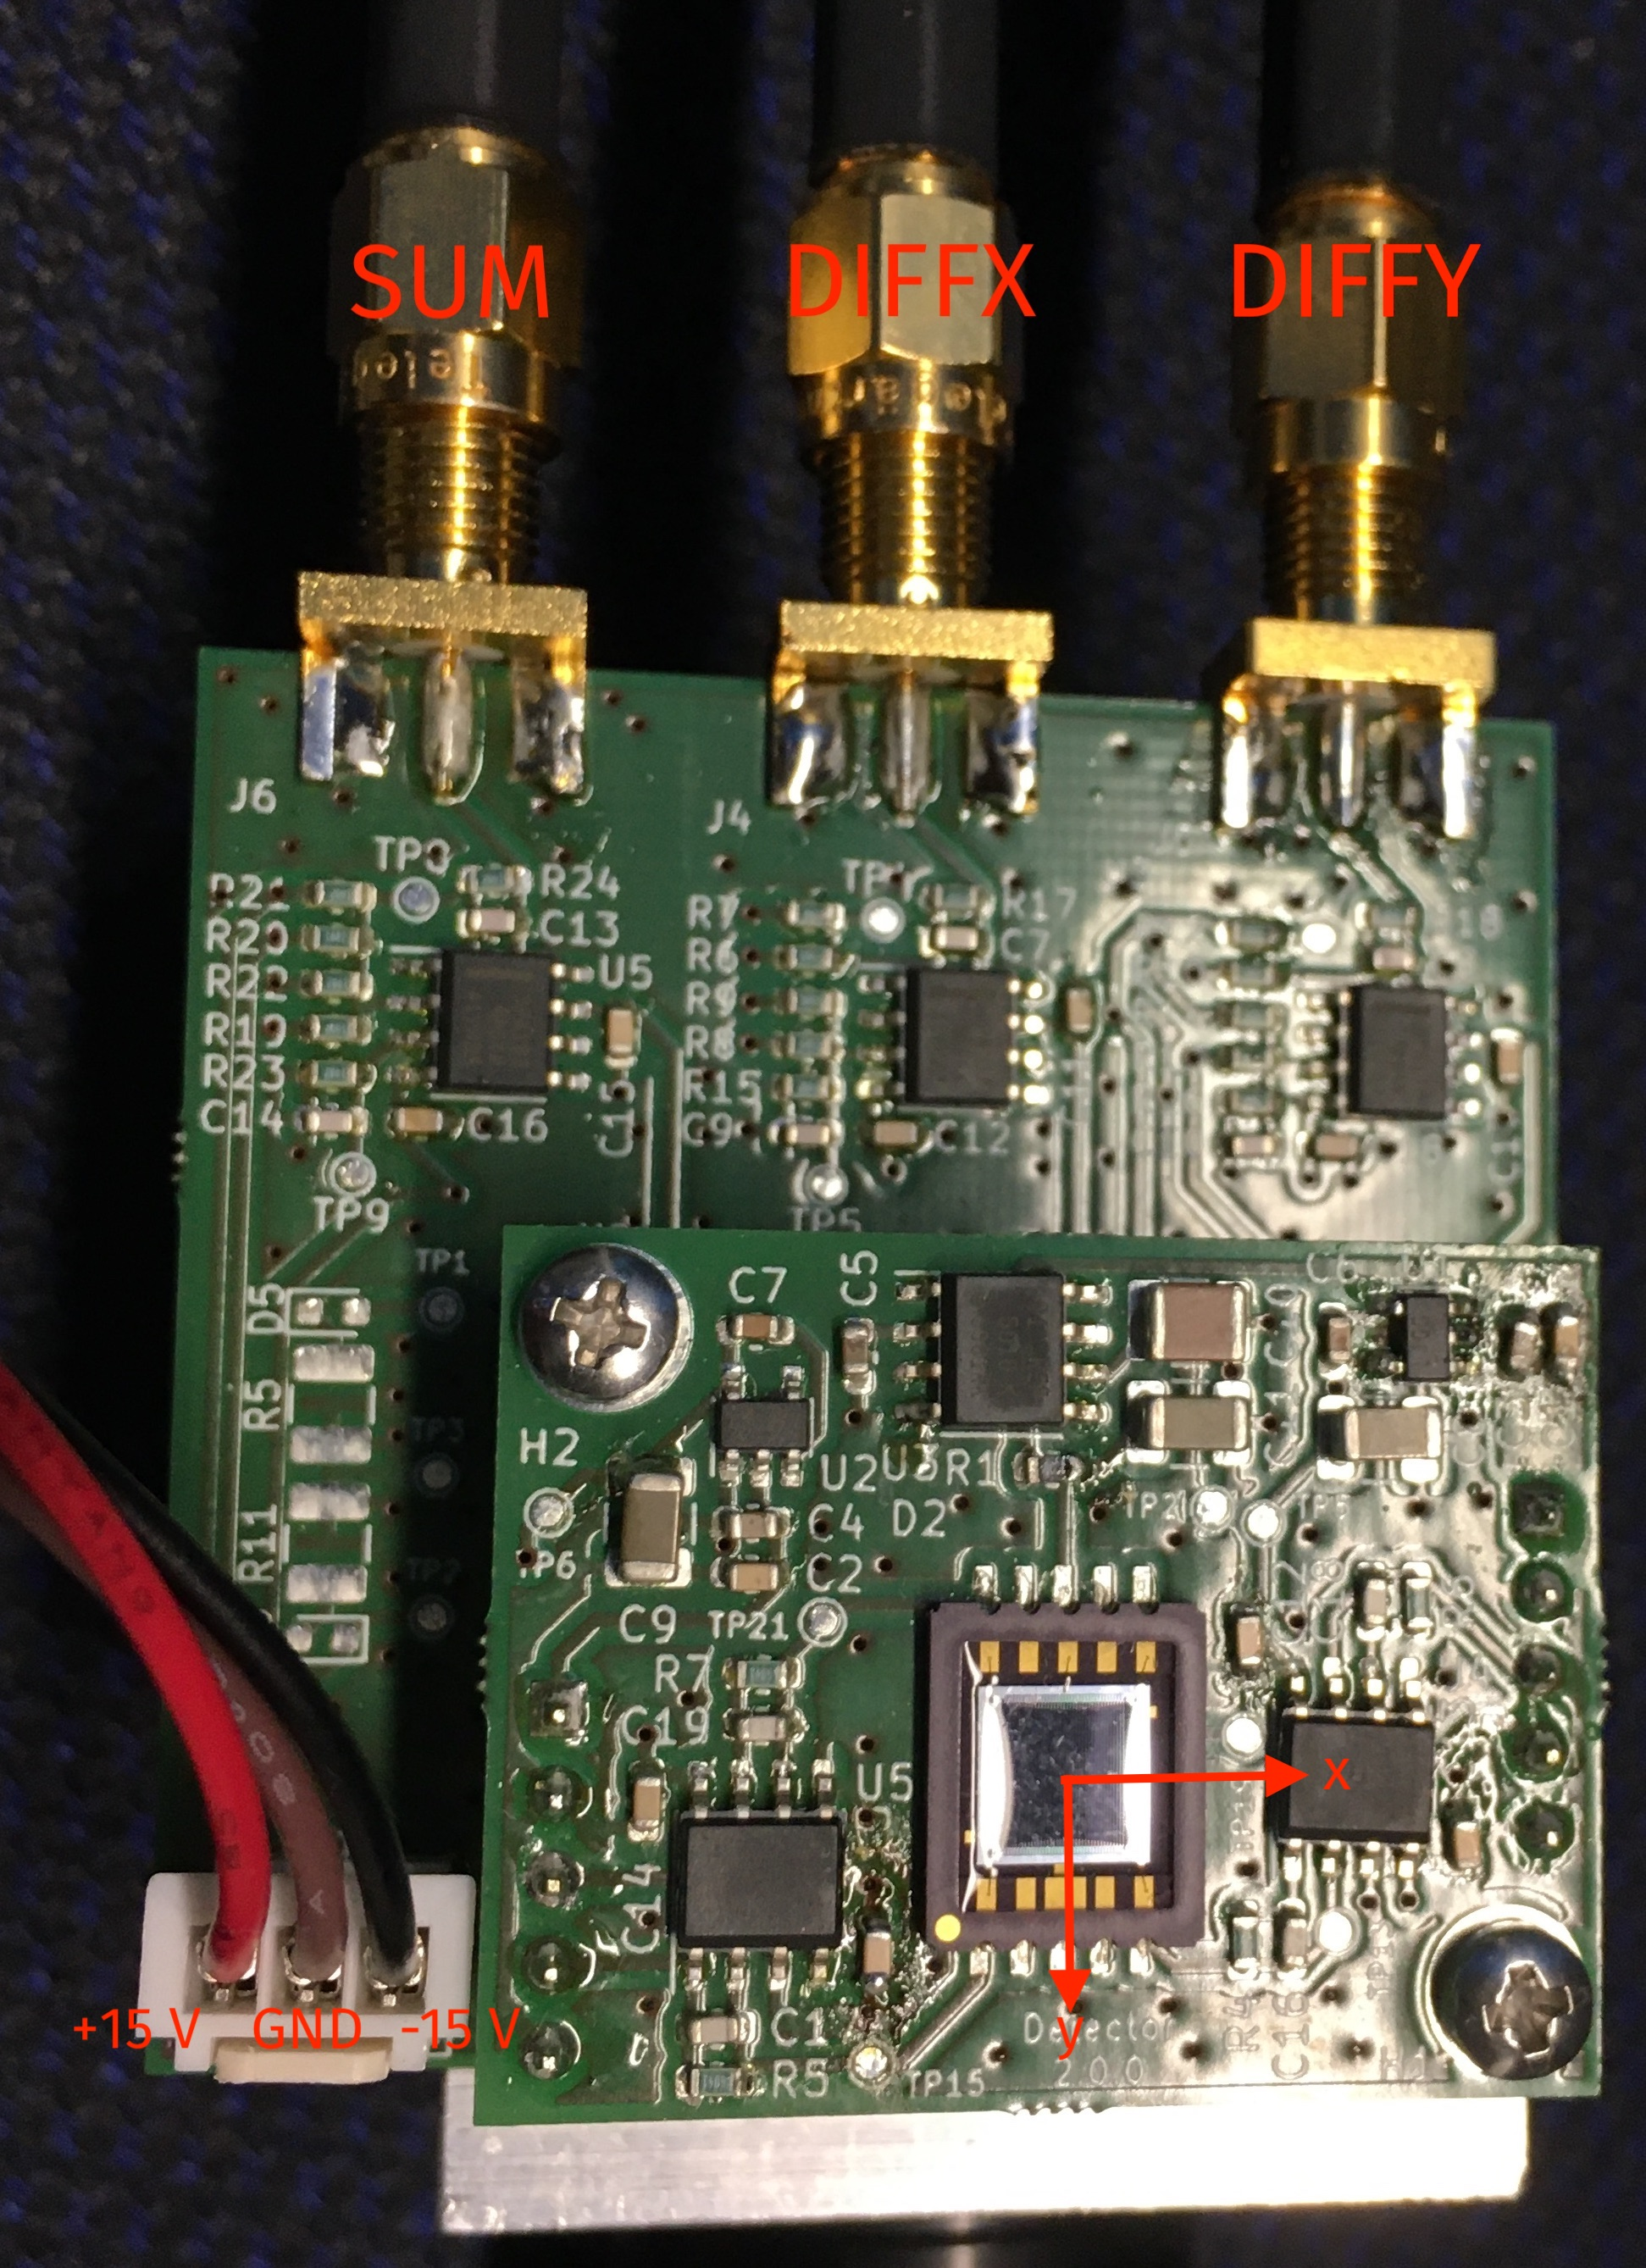
\includegraphics[scale=0.2]{detector.jpg}
	\caption{\gls{psd} on optical mount with connected cables}\label{fig:detector}
\end{figure}
\Cref{fig:detector} shows an image of the \gls{psd}.
The output voltage signals can be tapped from the upper \gls{sma} connectors.
The upper left connector gives the SUM voltage which reflects the total intensity of the optical signal.
The upper center connector gives the DIFFX voltage which reflects the difference proportional to the horizontal position on the sensitive area.
The upper right connector gives the DIFFY voltage which is proportional to the vertical position.
The SUM voltage is required to normalize the difference signals.
The DIFFX voltage increases when moving the light beam on the sensitive area to the right while the DIFFY voltage increases while moving the light beam to the bottom.
The device is powered by a 3-pin connector.
The outer (left) cable is the positive \SI{+15}{\volt} supply while the opposite cable is negative \SI{-15}{\volt} supply.
The center cable of the 3-pin connector has to reference ground.
The power connector has no polarity protection so be careful!

\begin{table}[htb]
  \centering
  \begin{tabular}{lcccc}
    \toprule
      Parameter & Minimum & Typical & Maximum \\
    \midrule
      Output voltages & \SI{-13}{\volt} & \SIrange{-2}{+2}{\volt} & \SI{+13}{\volt} \\
      Supply voltages & \SI{\pm13}{\volt} & \SI{\pm15}{\volt} & \SI{\pm37}{\volt} \\
      Spatial resolution & \SI{5.0}{\micro\meter} & \SI{2}{\micro\meter} & \SI{1}{\micro\meter} \\
      Bandwidth & & \SI{1400}{\kilo\hertz} & \\
    \bottomrule
  \end{tabular}
  \captionsetup{width=.8\textwidth}
  \caption{Specifications of the presented \gls{psd}}\label{tab:specifications}
\end{table}
\Cref{tab:specifications} summarizes the specifications of the presented \gls{psd}.
These specifications are only a rough estimate and we only assembled one \gls{psd} so far.
\section{Requirements}

\begin{enumerate}
    \item Dual power supply $V_\pm=\pm\SI{15}{\volt}$
    \item Ethernet network interface
    \item Spatial resolution $\Delta x=\SI{1}{\micro\meter}$
\end{enumerate}
\section{Position-sensitive detector}

The \gls{psd} constitutes the heart of the position-sensitive device.
Its characteristics give the upper bound of the performance of our device.
In the following section we will give an overview of the available methods for optical position measurement in order to motivate the selection of a tetra-lateral \gls{psd} photodiode.
The arguments given are an excerpt of Ref.~\cite{Noorlag74}.
To the end of this section we describe how the \gls{psd} can be integrated into the framework of electrical circuit analysis.

\subsection{Optical position sensors}

Position measurement can be encoded by frequency, amplitude, pulse and spatial modulation of an optical signal.
However, only spatial modulation of an optical signal encodes the position information of the plane transverse to the signal.
We can distinguish between three types of two-dimensional position sensors:
\begin{enumerate}
	\item Image detectors
	\item Quadrant detectors
	\item Position-sensitive detectors
\end{enumerate}
Image detectors typically consists of an array of a photo-sensitive detectors, therefore they are able to image precise spatial distribution of a signal.
However, because of their discrete nature they only have a low resolution with respect to the center-of-mass of the signal.
Quadrant detectors consist of four photodiodes in close proximity.
From the photocurrent of every respective photodiode one can calculate the center-of-mass of the signal.
With the quadrant detectors there is always a loss of signal in the spacing region between the photodiodes.
In comparison to the quadrant detectors the \gls{psd} consists of a single (lateral) photodiode.
Therefore we expect the \gls{psd} to provide the highest resolution with respect to the center-of-mass of the incident signal.

\subsection{Operating principle}

The operating principle of the \gls{psd} can be though as follows:
Photons of the optical signal excite electrons to the surface of the \gls{psd}.
These electrons will divide across the four \gls{psd} anodes according to the resistance.
For an ideal \gls{psd} the surface resistance is homogeneous such that the effective resistance from the center-of-mass of the optical signal to the respective \gls{psd} anodes is determined by the respective linear distance.
More precise the anode currents in one dimension $I_1,I_2$ are given by,
\begin{align}
	I_1=\left(\frac{1}{2}-\frac{x}{L}\right)\left(I_1+I_2\right), &&
	I_2=\left(\frac{1}{2}+\frac{x}{L}\right)\left(I_1+I_2\right),
	\label{eq:psd_anode_current}
\end{align}
wherein $x$ is the distance of the center-of-mass of the signal from the center of the \gls{psd}.
We can use \Cref{eq:psd_anode_current} to find the position $x$,
\begin{equation}
	x=\frac{L}{2}\frac{I_2-I_1}{I_1+I_2}
	\label{eq:psd_position_1d}.
\end{equation}
Analogue one obtains the positions in the two dimensional case from,
\begin{align}
	x&=\frac{L}{2}\frac{(I_{X2}+I_{Y1})-(I_{X1}+I_{Y2})}{I_{X1}+I_{X2}+I_{Y1}+I_{Y2}},\\
	y&=\frac{L}{2}\frac{(I_{X2}+I_{Y2})-(I_{X1}+I_{Y1})}{I_{X1}+I_{X2}+I_{Y1}+I_{Y2}}	
	\label{eq:psd_position_2d}.	
\end{align}
Fundamental to the derivation was the assumption that the surface resistance is homogeneous over the \gls{psd}.
In case of the older tetra-lateral \gls{psd} design this assumption is not really justified and the surface resistance shows a linear distortion.
Fortunately the modern design improved tetra-lateral (pin-cushion) \gls{psd} chooses an arrangement of the anodes to compensate for these non-linearities.

\subsection{Detector selection}

Given the previous information the obvious choice for our use case is a tetra-lateral \gls{psd} of the improved (pin-cushion) type.
At the time of writing there are two major manufactures of such \gls{psd} --- First Sensor and Hamamatsu.
Having said that only Hamamatsu sells its \gls{psd} in small quantities.
In \Cref{tab:psd_hamamatsu} we present the \gls{psd} portfolio of Hamamatsu.
\begin{table}[H]
	\centering
	\begin{tabular}{lccccl}
		\toprule
			Item designation & S1880 & S2044 & S5990 & S5991 & Unit \\
		\midrule
			Photosensitive area &
			\num{12.0 x 12.0} & 
			\num{4.7 x 4.7} & 
			\num{4.0 x 4.0} & 
			\num{9.0 x 9.0} & 
			\si{\milli\meter\squared} \\
		\bottomrule	
	\end{tabular}
	\caption{\gls{psd} portfolio of Hamamatsu.}\label{tab:psd_hamamatsu}
\end{table}
The S1880 and S2044 use a multi-zone design whereas the S5990 and S5991 use the preferable improved tetra-lateral (pin-cushion) design.
The S5990 and S5991 share the same design but differ in size and specifications.
The increase in size of the S5991 compared to the S5990 yields some more undesired electrical properties.
In general we can use an additional lens in front of the \gls{psd} in order to project arbitrary optical signals onto the \gls{psd} surface, therefore the benefits of a better electronic characteristic outweigh the smaller photosensitive area and we select the \gls{s5990} as our preferred \gls{psd}.

\subsection{Equivalent circuit}

\Cref{fig:psd_symbol} shows the abstract schematic symbol for a two-dimensional \gls{psd} with the four anode terminals on the right hand side and a common cathode terminal on the left hand side.
We can apply a reverse bias voltage to the common cathode terminal in order to reduce the response time of the \gls{psd}.
According to Ref.~\cite{Noorlag74,HamamatsuPSD} highest spatial resolution is achieved with no reverse bias --- the common cathode terminal connected to ground --- as the reverse bias voltage increases the dark current of the \gls{psd}.
\begin{figure}[H]
	\centering
	\begin{circuitikz}
		\draw (0, 0)
			node[ocirc, label=CC] {}
			to[short, -*] ++(1, 0)
			+(4, 1)
			node[ocirc, label=X2] {}
			to[photodiode] +(0, 1)
			to[short, *-] +(0, -1)
			+(4, 3)
			node[ocirc, label=X1] {}
			to[photodiode] +(0, 3)
			to[short, *-] +(0, -3)
			+(4, -1)
			node[ocirc, label=Y1] {}
			to[photodiode] +(0, -1)
			to[short, *-] +(0, 1)
			+(4, -3)
			node[ocirc, label=Y2] {}
			to[photodiode] +(0,-3)
			to[short, *-] +(0, 3)
	;
	\end{circuitikz}
	\caption{Equivalent circuit of one of the \gls{psd} output terminals according to~\cite{HamamatsuPSD}.}\label{fig:psd_symbol}
\end{figure}
That said, the representation of \Cref{fig:psd_symbol} is not very useful for practical calculations.
Instead we will model the output terminals of the \gls{psd} as a two current sources with internal resistance $R_i$ and capacitance $C_t$~\cite{HamamatsuPSD}.
Such an equivalent circuit is presented in \Cref{fig:psd_circuit}.
The first current source represents the photo current $I_p$ which is created from photons that excite electrons.
The second current source represents the dark current $I_d$ which is created from thermal excitation of electrons.
\begin{figure}[H]
	\centering
	\begin{circuitikz}
		\draw (-1, -1)
			node[ground] {}
			to[short] ++(0, 1)
			to[short] ++(1, 0);
		\draw (0, 3)
			to[american current source, label=$I_p$] +(4, 0);
		\draw (0, 1)
			to[american current source, label=$I_d$] +(4, 0);
		\draw (0, -1)
			to[european resistor, label=$R_i$] +(4, 0);
		\draw (0, -3)
			to[capacitor, label=$C_t$] +(4, 0);
		\draw (0, 0)
			to[short, -*] ++(0, 1)
			to[short] ++(0, 2);
		\draw (0, 0)
			to[short, -*] ++(0, -1)
			to[short] ++(0, -2);
		\draw (4, 0)
			to[short, -*] ++(0, 1)
			to[short] ++(0, 2);
		\draw (4, 0)
			to[short, -*] ++(0, -1)
			to[short] ++(0, -2);
		\draw (5, 0)
			node[ocirc, label=X] {}
			to[short, -*] ++(-1, 0);
	\end{circuitikz}
	\caption{Equivalent circuit of one of the \gls{psd} output terminals according to~\cite{HamamatsuPSD}.}\label{fig:psd_circuit}
\end{figure}
The parameters for the equivalent circuit of the \gls{s5990} are summarized in \Cref{tab:psd_s5990}.
If not stated otherwise we will use the maximum values from the datasheet.
\begin{table}[H]
	\centering
	\begin{tabular}{lllll}
		\toprule
			\multirow{2}[3]{*}{Parameter} &
			\multirow{2}[3]{*}{Symbol} &
			\multicolumn{2}{c}{Values} &
			\multirow{2}[3]{*}{Unit} \\
			\cmidrule(lr){3-4} & & Typical & Maximum & \\
		\midrule
		Dark current & $I_d$ & \num{0.5} & \num{10} & \si{\nano\ampere}\\
		Interelectrode resistance & $R_e$ & \num{7} & \num{15} & \si{\kilo\ohm}\\
		Terminal capacitance & $C_t$ & \num{150} & \num{300} & \si{\pico\farad}\\
		\bottomrule	
	\end{tabular}
	\caption{Important parameters of the \gls{s5990} extracted from the datasheet~\cite{HamamatsuS5990}.}\label{tab:psd_s5990}
\end{table}

\section{Transimpedance amplifier}

% TODO: motivate choice for current-to-voltage (transimpedance) design
% TODO: mention feedback tee network for high feedback factor

\begin{figure}[H]
	\centering
	\begin{circuitikz}
		\draw (0, 0) node[op amp](opamp){};
		\draw (opamp.+) -- +(0, -1) node[ground](gnd1){};
		\draw (opamp.out) -- (3, 0) node[ocirc, label=$V_\text{out}$]{};
		\draw (opamp.-) to[current source, invert, l=$I_\text{in}$] +(-3, 0) node(node1){} -- (node1 |- gnd1) node[ground]{};
		\draw (opamp.-) |- (-1, 2) to[resistor, l=$R_f$] (1,2) -| (opamp.out);
	\end{circuitikz}
	\caption{Simple transimpedance amplifier circuit.}
\end{figure}

\begin{equation}
	V_\text{out}=R_fI_\text{in}
\end{equation}

\begin{figure}[H]
	\begin{subfigure}[t]{.5\textwidth}
		\centering
		\begin{circuitikz}
			\draw (0, 0) node[op amp](opamp){};
			\draw (opamp.+) -- +(0, -1) node[ground](gnd1){};
			\draw (opamp.out) -- +(.5, 0) node[ocirc, label=$V_\text{out}$]{};
			\draw (opamp.-) -- +(-3, 0) node(node1){} to[current source, invert, l=$I_\text{in}$] (node1 |- gnd1) node[ground]{};
			\draw (node1) -- +(1.5, 0) node(node2){} to[resistor, l=$R_\text{in}$] (node2 |- gnd1) node[ground]{};
			\draw (opamp.-) |- (-1, 2) to[resistor, l=$R_f$] (1,2) -| (opamp.out);
		\end{circuitikz}
		\caption{Transimpedance amplifier.}
	\end{subfigure}
	\begin{subfigure}[t]{.5\textwidth}
		\centering
		\begin{circuitikz}
			\draw (0, 0) node[op amp](opamp){};
			\draw (opamp.+) -- +(0, -1) node[ground](gnd1){};
			\draw (opamp.out) -- +(.5, 0) node[ocirc, label=$V_\text{out}$]{};
			\draw (opamp.-) to[resistor, l_=$R_\text{in}$] +(-3, 0) node(node1){} to[voltage source, l=$V_\text{in}{=}R_\text{in}I_\text{in}$] (node1 |- gnd1) node[ground]{};
			\draw (opamp.-) |- (-1, 2) to[resistor, l=$R_f$] (1,2) -| (opamp.out);
		\end{circuitikz}
		\caption{Inverting amplifier.}
	\end{subfigure}
	\caption{Equivalence between transimpedance and inverting amplifier using source transformation.}
\end{figure}

\subsection{Noise}

% TODO: add shot noise
% TOOD: add thermal noise

\subsection{Offset}

% TODO: mention photodiode leakage current (Graemer p. 25)
% TODO: compensation circuit (Jung p. 57)

\subsubsection{Input current}

% TODO: mention that I+, I- are difficult to measure and therefore the datasheets report Ibias and Ioffset

\begin{figure}[H]
	\begin{subfigure}[t]{.5\textwidth}
		\centering
		\begin{circuitikz}
			\draw (0, 0) node[op amp, scale=1.2](opamp){};
			\draw (opamp.out) -- +(0.5, 0) node[ocirc, label=$V_\text{out}$]{};
			\draw (opamp.+) -- +(-0.5, 0) node(node1a)[circ]{} to[current source, l=$I_\text{offset}/2$] (node1a |- opamp.-) node(node1b)[circ]{} -- (opamp.-);
			\draw (node1a) -- ++(-1, 0) node(node2a)[circ]{} -- ++(0, -0.5) to[current source, l=$I_\text{bias}$] ++(0, -1) node[ground]{};
			\draw (node1b) -- ++(-1, 0) node(node2b)[circ]{} -- ++(0, +0.5) to[current source, l_=$I_\text{bias}$] ++(0, 1) node[ground, rotate=180]{};
			\draw (node2a) to[short, i<=$i_+$] +(-1.5, 0) node[ocirc, label=$V_+$]{};
			\draw (node2b) to[short, i<_=$i_-$] +(-1.5, 0) node[ocirc, label=$V_-$]{};
		\end{circuitikz}
		\caption{Equivalent current sources as reported in the datasheet.}
	\end{subfigure}
	\begin{subfigure}[t]{.5\textwidth}
		\centering
		\begin{circuitikz}
			\draw (0, 0) node[op amp, scale=1.2](opamp){};
			\draw (opamp.out) -- +(0.5, 0) node[ocirc, label=$V_\text{out}$]{};
			\draw (opamp.+)-- ++(-0.5, 0) node(node2a)[circ]{} -- ++(0, -0.5) to[current source, l=$I_-$] ++(0, -1) node[ground]{};
			\draw (opamp.-) -- ++(-0.5, 0) node(node2b)[circ]{} -- ++(0, +0.5) to[current source, l_=$I_+$] ++(0, 1) node[ground, rotate=180]{};
			\draw (node2a) to[short, i<=$i_+$] +(-1.5, 0) node[ocirc, label=$V_+$]{};
			\draw (node2b) to[short, i<_=$i_-$] +(-1.5, 0) node[ocirc, label=$V_-$]{};
		\end{circuitikz}
		\caption{Alternative equivalent current sources.}
	\end{subfigure}
	\caption{Non-zero input current from the operational amplifier.}
\end{figure}

\begin{align}
	I_+=I_\text{bias}+\frac{1}{2}I_\text{offset} &&
	I_\text{offset}=I_+-I_- \\
	I_-=I_\text{bias}-\frac{1}{2}I_\text{offset} &&
	I_\text{bias}=\frac{I_++I_-}{2}
\end{align}

\subsubsection{Input offset voltage}

\subsubsection{Offset compensation}

\subsection{Bandwidth}


\section{Power management}

\subsection{Input voltage}

% checkout Henry Ott's filter suggestions

\subsubsection{Reverse polarity protection}

% reference https://www.edn.com/design/power-management/4433697/Protecting-against-reverse-polarity--Methods-examined--Part-1
% describe MOSFET + Schottky solution

\subsubsection{Capacitance multiplier}

\subsection{Internal power supply}

\subsubsection{Dual supply voltage regulator}

\subsubsection{High-precision voltage reference}
\section{Printed circuit board}

% References:
% - Henry Ott

% Formula for track width, depth

% Terminology (maybe just as glossary?):
% - Tracks
% - Vias
% - Cooper fill / pour
% - Solder pads

\subsection{Layout and stackup}

% Signal - Ground - Ground - Signal (Ott p. 641)

\printglossaries
\printbibliography
	
\end{document}